% Notas del integrante 2. Compilar notas/main.tex.
\section*{\personaDos · gRPC}
\small
\textbf{Proyecto}\quad \proyectoDos\par
\subsection*{Teoría y ejemplo sencillo}
gRPC define el servicio en un archivo \texttt{.proto}; de ese contrato se genera el stub del cliente y la base del servidor, y los mensajes viajan en binario con Protocol Buffers sobre HTTP/2 \cite{kaminski2023}. En la demo, \texttt{ClienteTurnos} hace el papel de Inspecciones y llama a \texttt{ConsultarTurno} en \texttt{ServidorTurnos}, que hace el de Turnos y Pagos. Con la placa \texttt{GSA-1234} respondió \texttt{CONFIRMADO}; con \texttt{MBA-0567}, \texttt{PENDIENTE\_PAGO}; con \texttt{XYZ-999}, \texttt{SIN\_TURNO}; y con el servidor apagado el cliente recibió \texttt{UNAVAILABLE} (capturas en \path{evidencias/integrante-2/demo-grpc/}).
\subsection*{Aplicación futura al proyecto}
\textbf{Estado actual.} El prototipo del PFC separa Inspecciones y Turnos y Pagos, cada uno con Spring Boot y su propia base PostgreSQL, y los comunica por REST con \texttt{POST /turnos/\{id\}/autorizaciones-inspeccion}. El equipo midió un p95 de 47,4 ms con 10 usuarios en un equipo local \cite{rtvpfc2026}. \textbf{Supuesto de diseño, no es el estado actual:} llevar esa llamada a gRPC unario y bloqueante con un \emph{deadline} de 3 s, que es el mismo límite que hoy usa REST. Ofrece transparencia de acceso, pero no de fallos. Ante un corte se prioriza la consistencia: sin autorización no se inicia la inspección. Con la red sana también se prioriza la consistencia, porque debe existir una sola autorización por turno. La mejora en latencia no está medida.
\subsection*{Fallo supuesto y conclusión}
Si la autorización se guarda pero la respuesta llega tarde, el cliente recibe \texttt{DEADLINE\_EXCEEDED} aunque el servidor ya escribió \cite{grpcdeadlines}. Por eso el reintento debe llevar la misma clave de idempotencia, como hace Stripe \cite{stripeidempotency}. Antes de cambiar REST por gRPC, implementaría esa clave en el contrato y la validaría demorando el servidor más de 3 s para comprobar que queda una sola autorización.

\begin{minipage}{\linewidth}
\textbf{Anexo: bosquejo a mano}\par\smallskip
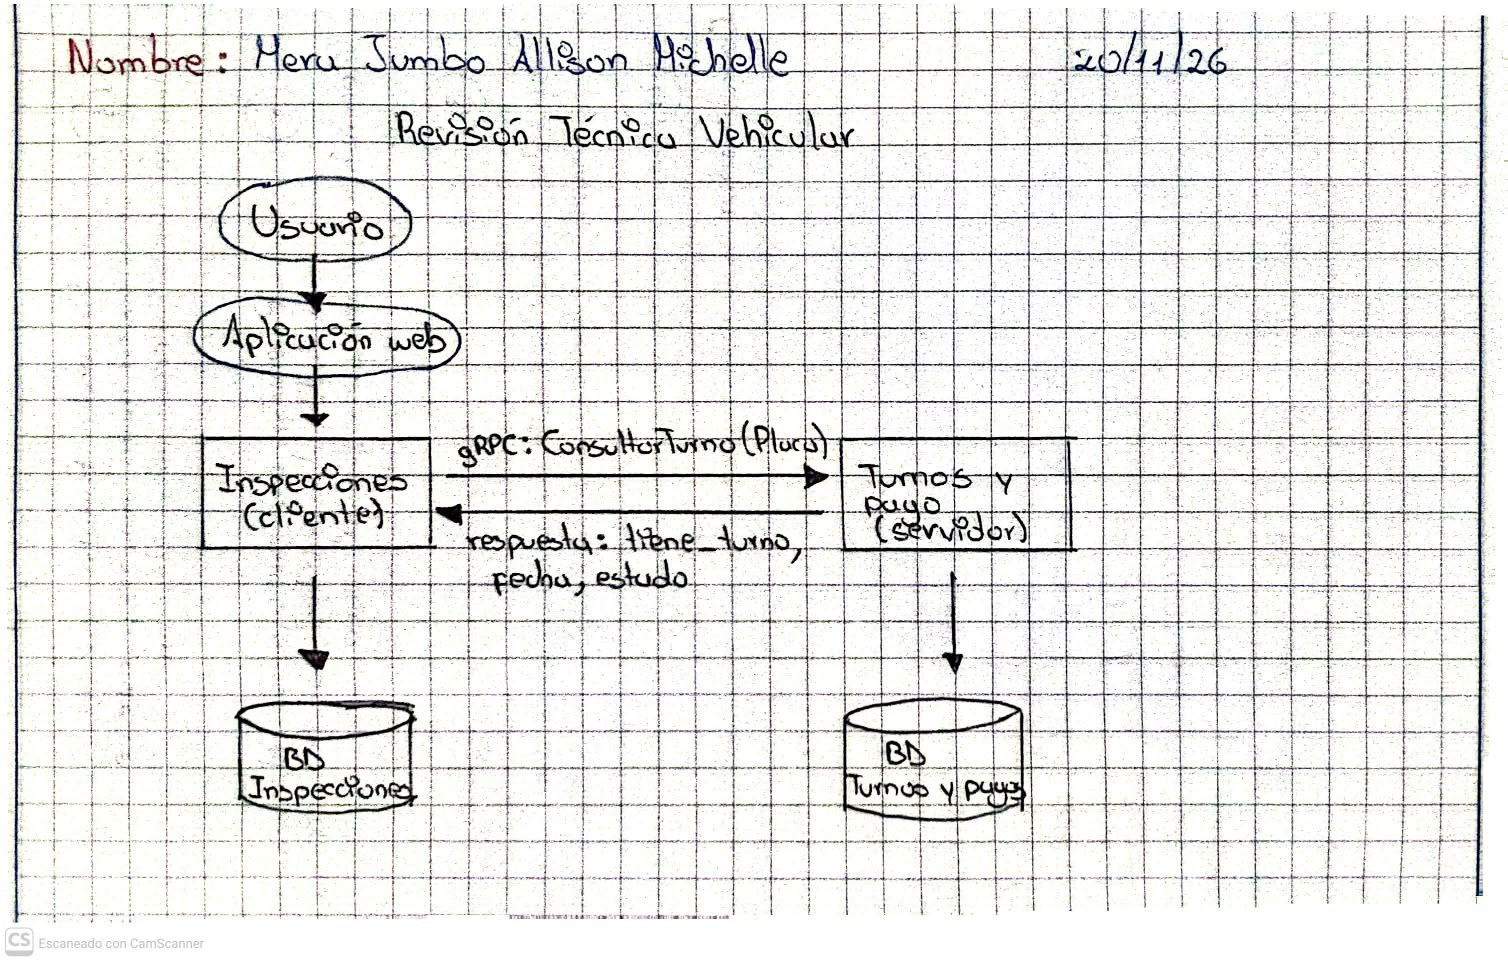
\includegraphics[height=.2\textheight,keepaspectratio]{../evidencias/integrante-2/esquema-mano/esquema-mano-revision-vehicular-grpc-2026-11-20.jpeg}\par
{\footnotesize Bosquejo original de \personaDos, 20 de noviembre de 2026. Vista parcial del RTV: solo la autorización de inicio; la llamada gRPC es supuesta.}
\end{minipage}